\section[Future Work]{Future Work}
\label{sec:future}

\begin{frame}{Future Work}
The grid analyzed for online/real-time analysis should be bigger, in order to demonstrate spatial variation in the early warning sign indicators for different buses/areas and for singling out areas which are more vulnerable to steady state instabilities.

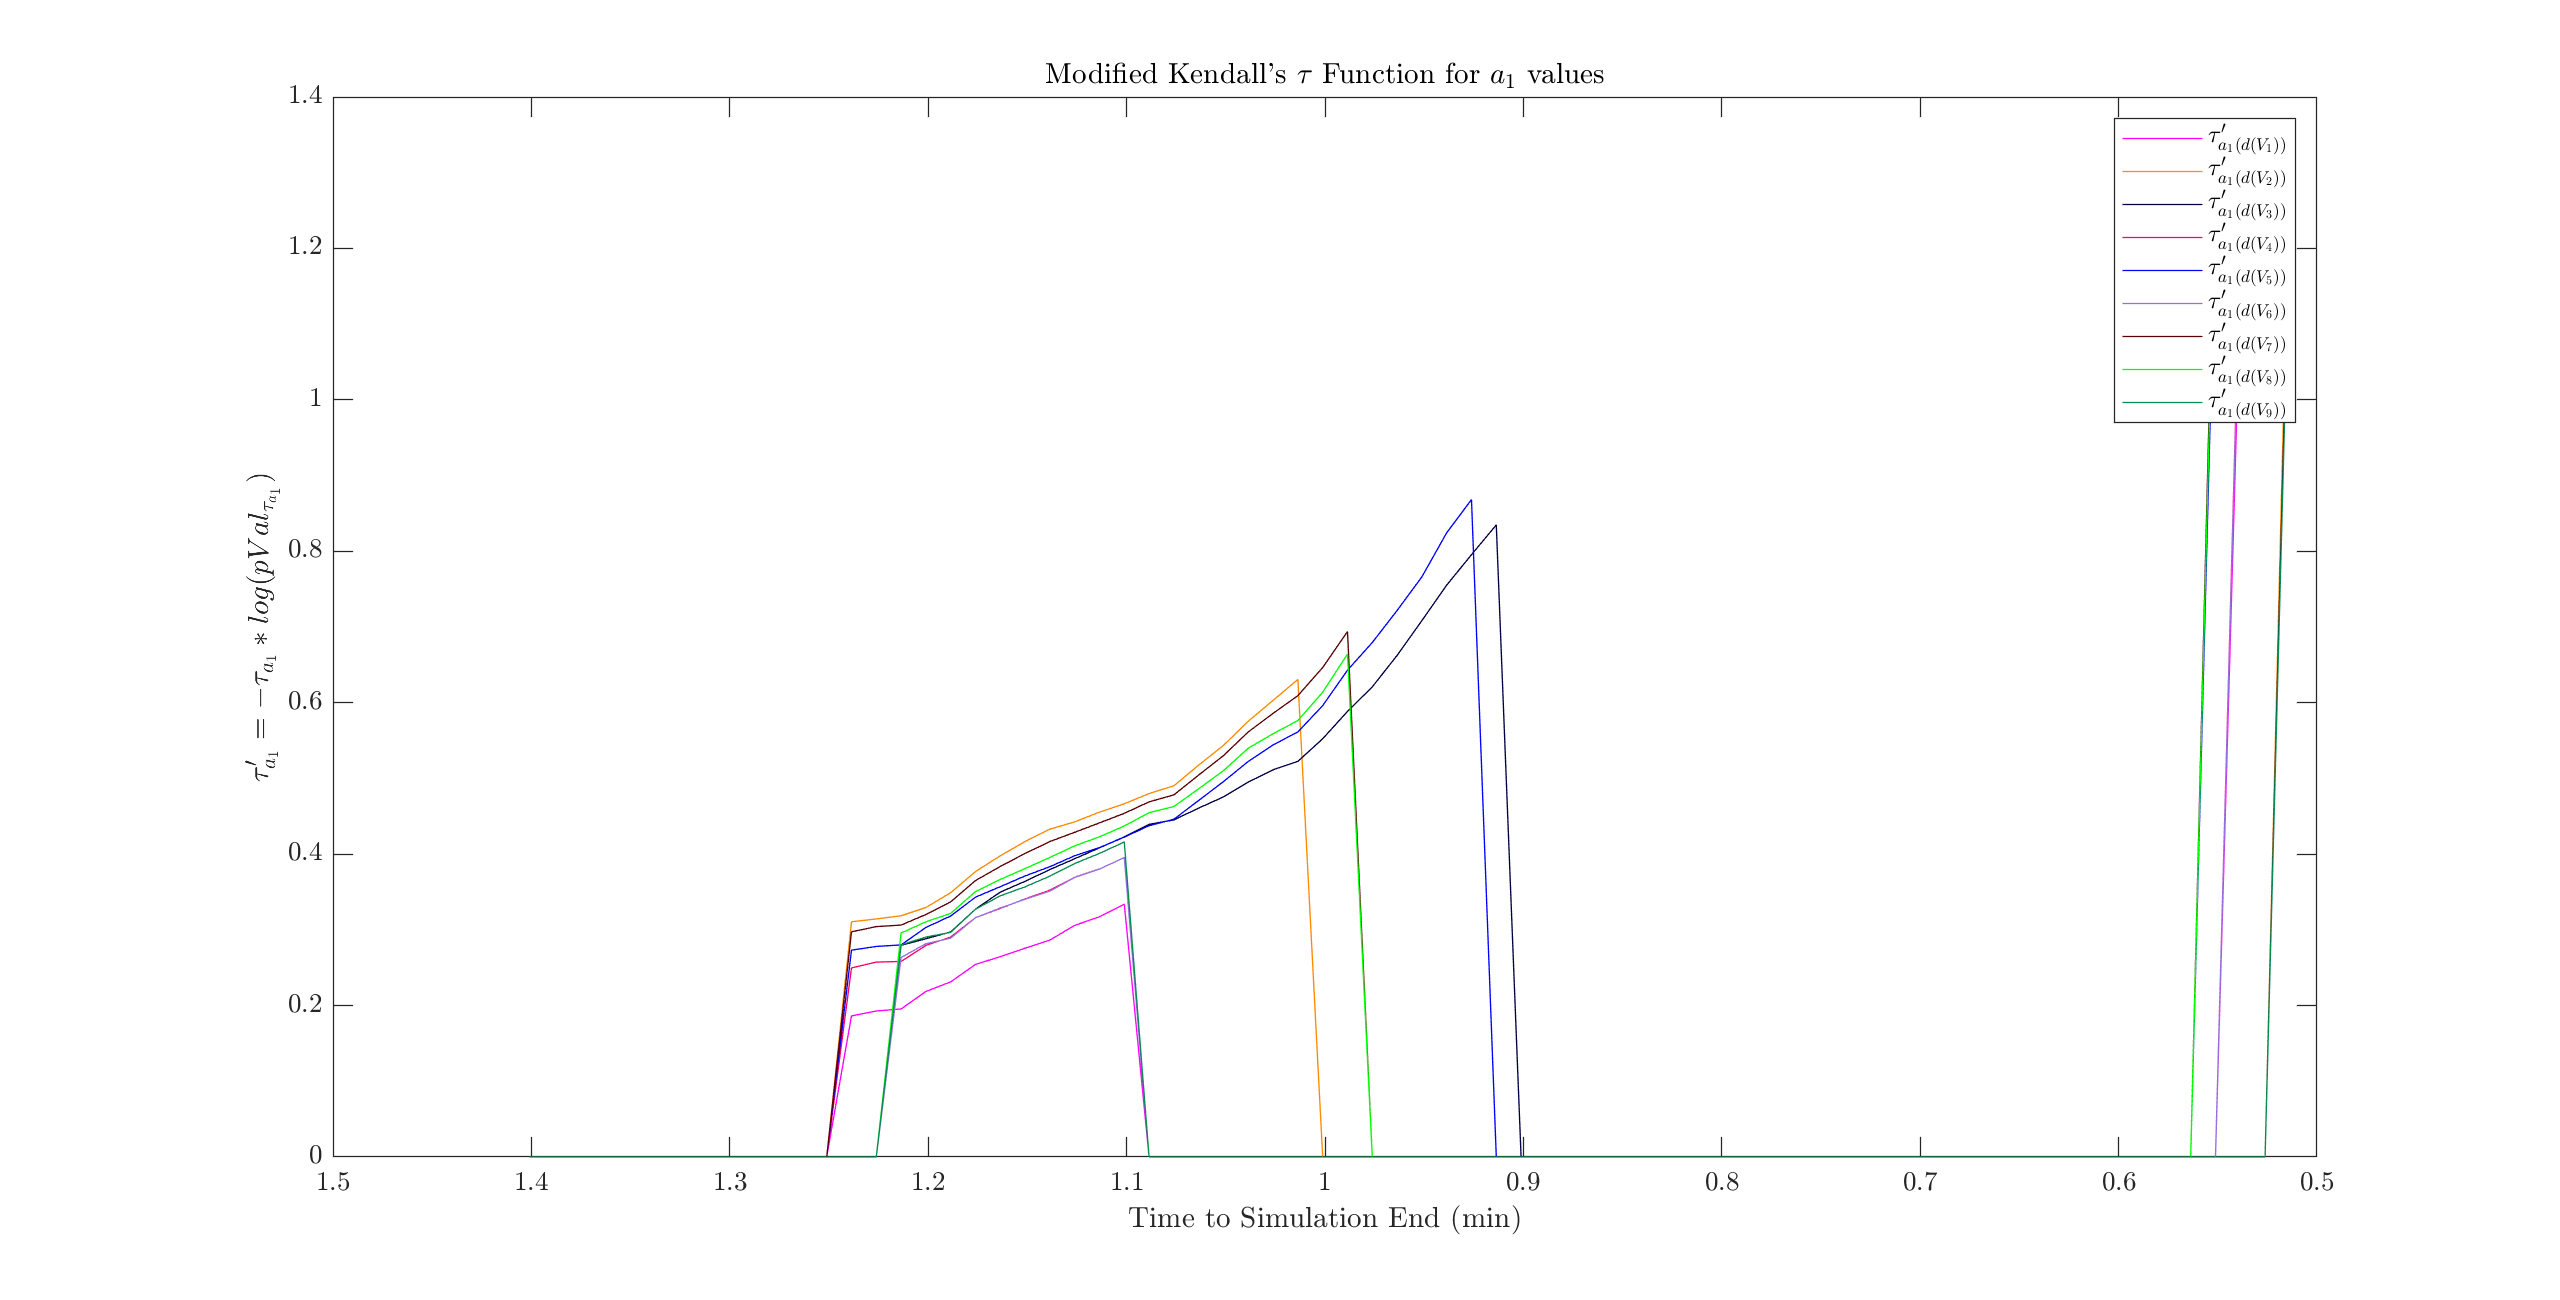
\includegraphics[scale=0.15]{../figures/im03.png}
\end{frame}

\begin{frame}{Future Work}
Despite the successful application of statistical analysis to detect symptoms of Critical Slowing Down in various phenomena \cite{schefferEarlyWarningSignalsForCriticalTransitions}, autocorrelation and variance are not certain indicators for the same, at least by themselves \cite{csdNotDetectedByAutocorrAndVariance01}.
In order to tackle that, statistical parameters other than autocorrelation and variance can be investigated for their feasibility as Early Warning Signal indicators. Even for the same statistical indicators, changing the length of the running window, time lag $\tau$, sampling rate etc. can have a significant effect on their effectiveness. Thus an `optimal' set of parameters could be researched for, which may be different for different grids, but shouldn't vary for a particular grid once computed.
On similar lines, grid state variables other than bus voltages, line current/MVAs, grid frequencies may be investigated.
\end{frame}
